% \section{Large-scale Empirical Study and Discoveries}
\chapter{仿冒应用基本特征解读}
\label{chp:discoveries_basic}

上一章节介绍了本研究的相关设置,提出了7个与仿冒应用相关的研究问题。
本章从仿冒应用与原版应用相似度、影响仿冒应用数量的因素及仿冒应用行为三点入手,回答与仿冒应用基本特征相关的三个研究问题,即:

\noindent{\bf RQ1:仿冒应用和与之相对的正版应用的相似程度如何?}
\noindent{\bf RQ2:正版应用的热度、类别等因素是否会导致其吸引仿冒应用开发者对其进行仿冒?}
\noindent{\bf RQ3:仿冒应用作者制作出了怎样的仿冒应用?是否依然能提供原版应用的功能?}

\section{度量指标选择}

为回答RQ1,本研究需要选择一种相似度指标衡量仿冒应用与原版应用的相似程度;
为回答RQ2,需要先选择一种指标衡量某款应用在仿冒应用开发者眼中的受欢迎程度,再将其与可代表应用热度、应用类别的指标相关联,以计算两者间的关联性。

\vspace{0.5mm}
\noindent {\bf 相似程度度量指标}
\vspace{0.5mm}

应用之间相似度可从多个层面定义,包括应用行为相似度,应用代码相似度以及应用外观相似度。
应用行为相似度量度需要案例与一定方式驱动样例(常用的为手动方式驱动,或利用UI Automator或Monkeys等工具预先录制好操作脚本再回放)。
考虑到采集到的的应用规模较大,且种类繁多,要对逐个应用设计、驱动样例的可行性并不高,因此本研究不对所有应用进行行为相似度比对。
应用代码相似度比对常用于重打包检测相关研究,核心为对两个应用间的代码进行比较,计算两者间重合范围。
然而,仿冒应用的意图为诱导用户下载安装,而代码层面的内容不在普通用户的可感知范围内。
因此,仿冒应用代码并不需要与原版应用相似,代码相似度不是在本研究场景下最为重要的相似度指标。
进一步推断可得,外观相似度是最符合本研究场景的相似度类别,仿冒应用开发者甚至可以重新开发与原版应用外观相似的应用骗取用户下载。
根据日常经验,用户对应用外观的可感知的因素有以下几点:应用图标、应用GUI界面、应用标题(包括包名与应用名)和应用大小。
基于采集到的数据,本研究利用应用标题与应用大小进行相似度比较。

在文本相似度比对方面,本研究采用\textit{编辑距离}~\cite{levenshtein1966binary}作为具体度量指标。
编辑距离是在自然语言处理(Natural Language Processing,简称NLP)领域被广泛应用的距离定义,其定义如下:

\begin{Def}
    编辑距离

    给定两个字符串$a$与$b$,其间的编辑距离$d(a, b)$为将$a$和$b$相互转换的最小编辑操作数。
    其中,每次添加、删除或将一个字符转换成另一个字符均算作一次编辑操作。
\end{Def}

例如,``jingdong''和``jindeng''之间的编辑距离是2,由前者转换为后者的其中一种编辑次数最小方法为将第一个``g''删除,再将``e''转成``o''。
同理,字符串``fake''和``official''之间的距离是7,其中一种方案为在``f''前添加``o'',在``f''和``a''之间添加``fici''(此处包含4步操作),将``k''替换作``l'',最后删去``e''。

\vspace{0.5mm}
\noindent {\bf 关联程度度量指标}
\vspace{0.5mm}

本研究在衡量某款应用在仿冒应用开发者眼中受欢迎程度时,采用了较为直观的指标:从直觉上看,市面上存在越多仿冒个体的应用,越受仿冒应用开发者欢迎。

但是,每款目标App都有不同的样本数(官方样本数与仿冒样本数均有区别),所以不能直接以仿冒样本的数量作比较。
为了消除偏差,本文将样本数量归一化,使用仿冒率对比每个目标App在仿冒应用开发者中的受欢迎程度。

\begin{Def}
    仿冒率

    某款App~$a$的仿冒率$fake~sample~rate_a$指与其关联的仿冒样本的数量$fake_a$与该App正版样本的数量$total_a$的商;某应用市场$AS$的仿冒率$fake~sample~rate_{AS}$则是其中包含的所有目标App的均值。
    两者可分别计算如下:
\end{Def}

\begin{equation}
    fake~sample~rate_a = \frac{fake_a}{total_a} \,,
    \label{equ:fake_rate_app}
\end{equation}
\begin{equation}
    fake~sample~rate_{AS} = Avg(fake~sample~rate_a, \forall a \in \text{\{目标App\}}) \,.
    \label{equ:fake_rate_mkt}
\end{equation}

为探究应用受仿冒应用开发者的欢迎程度与其他因素的相关性,本研究利用皮尔逊积矩相关系数来计算一款App被仿冒的严重程度与其热度是否具有相关性。

\begin{Def}
    皮尔逊积矩相关系数

    两个变量之间的皮尔逊相关系数定义为两个变量之间的协方差和标准差的商,计算公式如下:
\end{Def}
\begin{equation}
    p_{x,y} = corr(X,Y)=\frac{cov(X,Y)}{\sigma_x\sigma_y}=\frac{E[(X-u_x)(Y-u_y)]}{\sigma_x\sigma_y} \,.
    \label{equ:PPMCC}
\end{equation}

\section{解读过程与结果}

\subsection{仿冒样本与原版应用的相似度研究}

\noindent{\bf RQ1:仿冒应用和与之相对的正版应用的相似程度如何?}

先从统计数据入手探索数据:
包名方面,应用数据集统计结果显示,在所有的52,638个仿冒样本中,只有243个(少于0.5\%)使用了正版应用的包名,余下的所有仿冒样本都使用了自定义包名。
自定义包名的52,395个样本中,包含了14,089个不同的包名。
应用名方面则有截然不同的结果,大部分样本(41,863个,约79.5\%)使用了与原版应用一致的应用名,余下10,775个仿冒应用样本包含应用名共10,610个。
绝大部分仿冒应用并未保留原版应用的包名,但只有较少仿冒应用采用了新应用名。

作者推断,仿冒样本之所以极少直接沿用正版应用的包名,很可能与Android系统机制有关。
根据Android官方文档~\cite{setAppId}描述,每个Android应用都具备一个名为Application ID的属性,该属性为Android系统用于识别应用程序的唯一标识。
通常情况下,该属性与包名一致。
如果系统在安装App时发现系统中已经有具有相同Application ID的App,将检查两个应用的应用证书是否一致,证书不一致会导致安装失败。
因此大部分仿冒应用不会直接使用正版App的包名。
而应用名只有向用户展示的用途,不用于系统内的应用校验,系统也允许出现重复的应用名,所以大部分仿冒应用采用了与原版应用一致的签名以更好地诱导用户下载。

之后,研究采用如上节所述的外观相似度衡量指标,比对原版应用与仿冒应用之间的相似程度。
对于从仿冒样本中获取到的每个应用名,均计算与其对应的官方发布App的原版应用名的编辑距离;
同理,也计算出每个仿冒样本包名与原版包名的编辑距离,结果可见下图~\autoref{fig:Statistic_fake_and_official}。

\begin{figure*}[htbp]
    \centering
    \subfloat[应用名\label{fig:appname}]{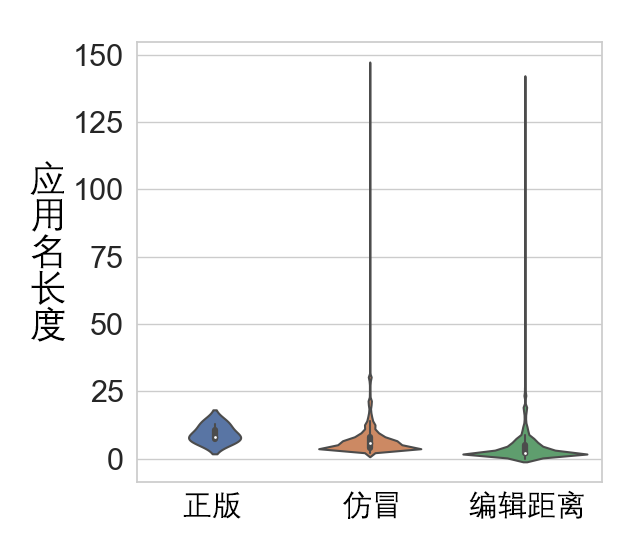
\includegraphics[width=0.333\textwidth]{./Figures/edwin-RQ1-2(a).png}}\hfill
    \subfloat[包名\label{fig:pkgname}]{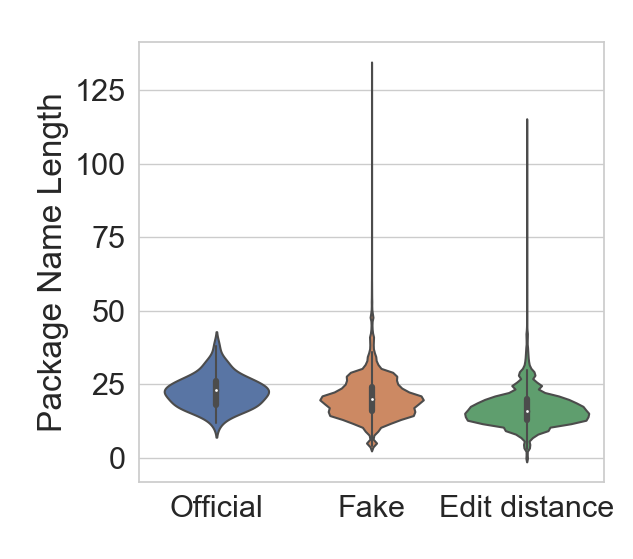
\includegraphics[width=0.333\textwidth]{./Figures/edwin-RQ1-2(b).png}}\hfill
    \subfloat[样本大小\label{fig:size}]{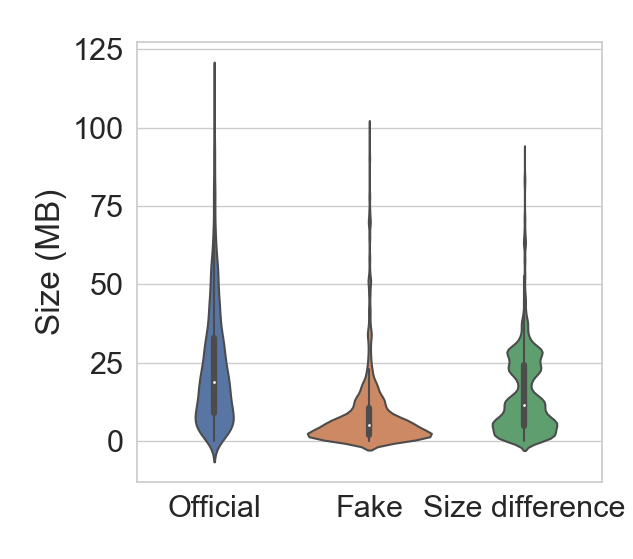
\includegraphics[width=0.333\textwidth]{./Figures/edwin-RQ1-2(c).png}}\hfill
    \caption{应用的应用名、包名与应用大小的相似性比较}
    \label{fig:Statistic_fake_and_official}
    \vspace{-5mm}
\end{figure*}

\autoref{fig:Statistic_fake_and_official}由三个小提琴图~\cite{violinplot}组成,分别表示了本文在应用名、包名和APK包大小上的统计信息。
每个``小提琴''的外部形状为数据的密度分布情况,小提琴中间的黑色粗条表示四分位数范围,粗条中小白点表示数据的中位数,黑色细条表示95\%置信空间范围。

\autoref{fig:appname}从左到右的三个图例分别展示官方样本、仿冒样本的应用名和两者间编辑距离的统计数据。
其中``正版''图例和``仿冒''图例中的中位数标志都接近数值``6'',说明官方样本和仿冒样本的应用名的平均长度十分相近。
``仿冒''图例整体分布具有集中性,较多样本分布在$y$轴数值为4到5之间,说明较多仿冒样本应用名长度落于此区间内。
``编辑距离''图例外部形状与``仿冒''图例大致类似,中位值十分低(在$y$轴上为``2''),意味着过半数仿冒应用通过从官方App的应用名中修改少于3个字符来获得其应用名。
上述结果表示大部分仿冒应用正在使用与官方App非常相似的应用名。
将三个图例与前文统计数据结合,可推断具备不同应用名的10,775个仿冒样本多数在原版应用名的基础上删减少量字符以获得新应用名。
同时,极少量仿冒应用有着异乎寻常的长名称(11个仿冒样本的应用名长度大于50个字符,最长的仿冒样本的应用名中甚至有146个字符)。
作者认为这部分异常样本可能是出于测试市场审查机制的目的被上传的。
此外,作者对部分具有长应用名的仿冒样本进行人工检查,一些长应用名拼合了多个热门App的名称(比如``潮流女装-美丽说蘑菇街淘宝天猫京东美团精选''或``老黄历万年历日历-农历天气预报知乎倒数日记账事本闹钟备忘录优步滴滴打车同花顺大智慧微博大众点评小说壁纸'')。
这可能是为了应用更容易地被用户搜索到而采取的策略。

\autoref{fig:pkgname}显示了针对包名的结果。
官方App的包名长度中位值和仿冒样本的包名长度中位值较为接近(双方的值分别为``23''和``20''),两者外形较为近似,说明原版样本与仿冒样本在包名长度上有类似分布。
然而,原版包名与仿冒样本包名之间编辑距离的中位数明显较高(在$y$轴上``16''的位置),这意味着将一个仿冒应用的包名转换为一个官方App的包名平均需要进行16次编辑。
换言之,官方App的包名和仿冒应用的包名有明显差异,仿冒应用更倾向于使用自定义且与原版应用有较大区别的包名。

\autoref{fig:size}则显示APK包大小的相关对比。
为了能更好地显示结果,部分极端样本在作图前被剔除出数据集:该部分样本为大于150MB的APK包,在所有69,614个官方App的样本中占851个(约为1\%),在52,638个仿冒样本中占447个(少于1\%),大部分来源于``游戏''类别下。
图表显示,仿冒样本大小的中位数约为5MB,约半数的正版App大小大于18MB。
``正版''图例中,应用大小样本分布相对均匀,密度曲线变化平缓,大部分样本分布于$(0, 60)$MB区间内,多数正版应用大小小于25MB,但在大于25MB的区间内仍有少量样本分布;
与之相比,``仿冒''图例的样本分布集中于3到4MB处,几乎没有样本大小大于25MB;
从该角度看,仿冒应用更有可能:

1) 由仿冒开发者自行开发,而非使用重打包技术制作。因为重打包之后的应用通常不会在大小上与原版有太大差距;

2) 是恶意应用。单独的恶意应用不需要包括较大的资源文件,只需少量具备恶意代码即可产生恶意行为;

\vspace{1mm}

简而言之,可从\autoref{fig:Statistic_fake_and_official}中获得两点总结,回答RQ1:

1) 更倾向于使用与正版App相似(甚至相同)的应用名,但包名与正版应用相差较大;

2) APK大小通常较小,很可能为仿冒应用开发者重新开发的恶意应用。
\vspace{1mm}


\begin{figure*}[t]
    \centering
    \subfloat[360应用市场\label{fig:360_detail}]{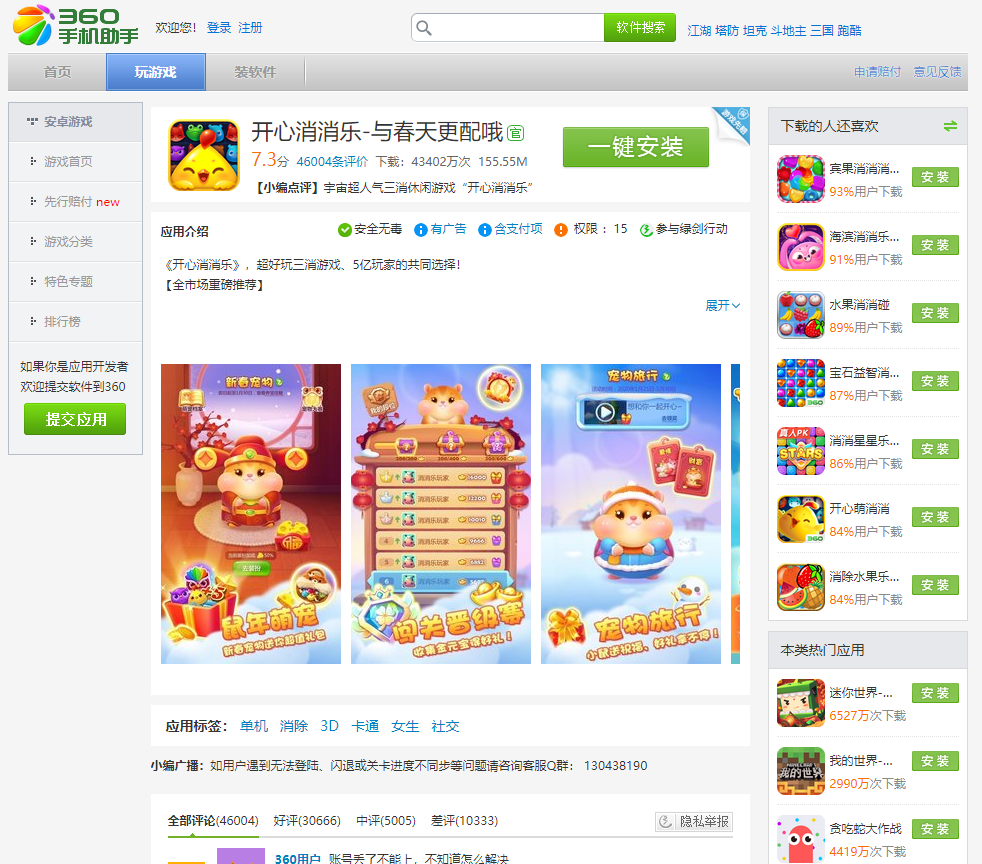
\includegraphics[width=0.49\textwidth]{./Figures/edwin-app-detail-360.png}}\hfill
    \subfloat[应用宝\label{fig:yyb_detail}]{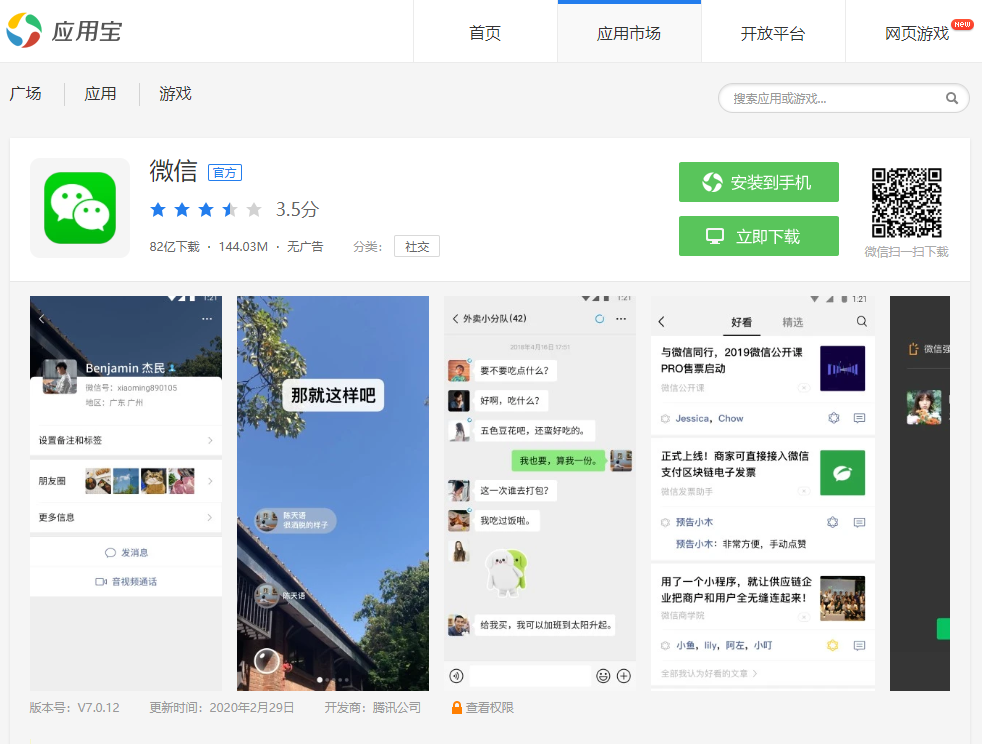
\includegraphics[width=0.49\textwidth]{./Figures/edwin-app-detail-yyb.png}}\hfill

    \subfloat[百度手机助手\label{fig:baidu_detail}]{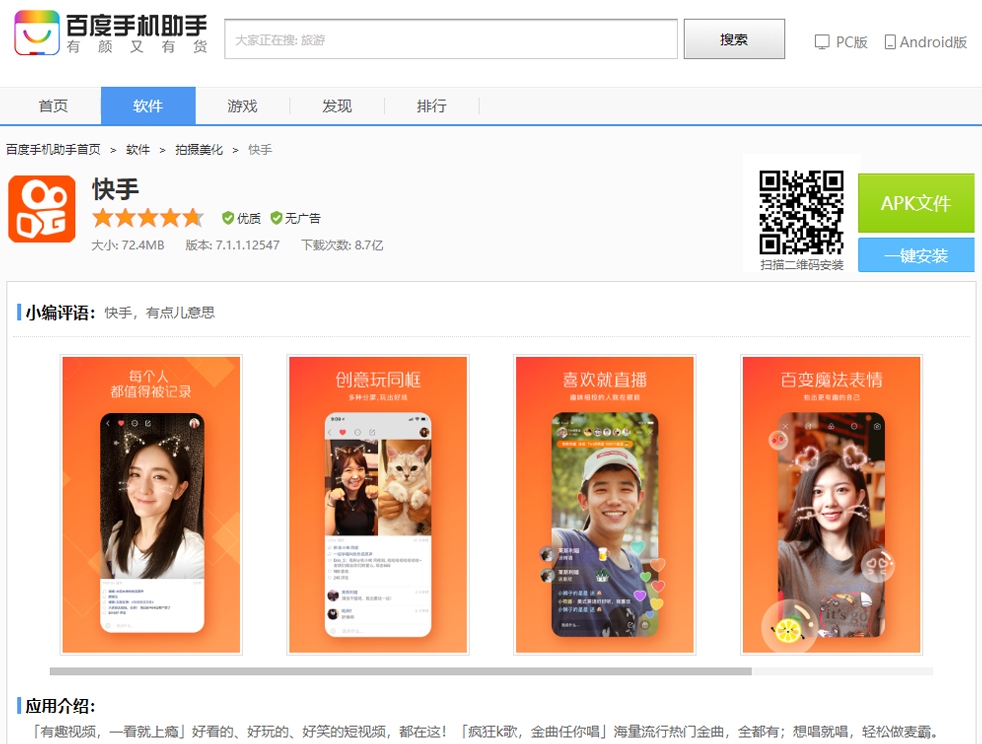
\includegraphics[width=0.49\textwidth]{./Figures/edwin-app-detail-baidu.png}}\hfill
    \subfloat[小米应用市场(部分信息被折叠)\label{fig:xiaomi_detail}]{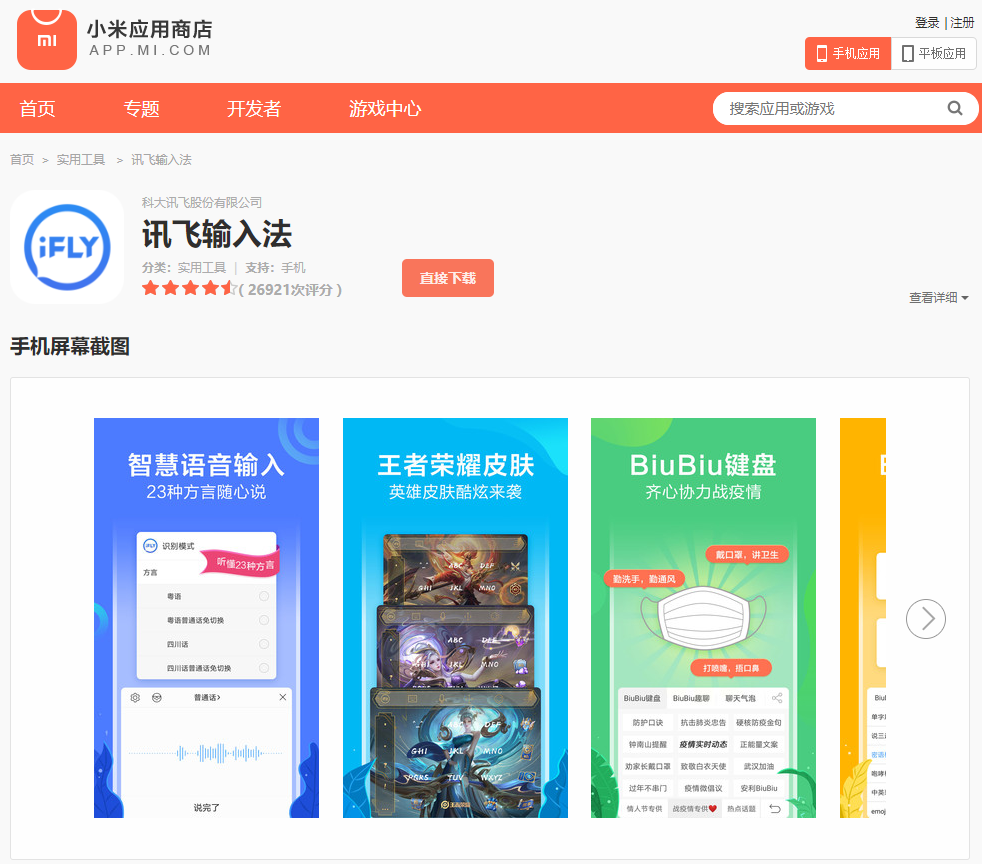
\includegraphics[width=0.49\textwidth]{./Figures/edwin-app-detail-xiaomi.png}}\hfill
    \caption{各大应用市场应用详情页}
    \label{fig:app_detail_page}
    \vspace{-5mm}
\end{figure*}

作者认为,造成上述第一点总结的原因是应用市场上提供的应用信息的不完备和用户对Android App了解的缺乏。
\autoref{fig:app_detail_page}显示了4个国内主流应用市场的详情页。
当用户浏览应用详情页时,各应用市场均显示对应应用的应用名、下载量、应用描述、其他用户对应用的评论和评分等信息。
但是,页面上较为醒目的条目是应用名、应用评分和图标信息,应用的技术参数(比如应用大小、版本号等)信息或是在不显眼处标记,或是被折叠,甚至不被展示。
在\autoref{fig:xiaomi_detail}所示的小米应用市场上,用户不能直接看到应用大小信息,需要点开折叠页才能获得相关数据。
上述四个应用市场应用详情页均不显示应用的包名信息。
由于普通用户不了解Android App中包名和应用名的区别和关联,展示相关信息对市场方引导用户下载安装应用也没有促进作用,市场对应用的技术参数展示并不重视。
因此,用户在应用市场上无法感知应用包名甚至应用大小,仿冒应用开发者无需在该两点上花费精力模仿正版应用。
相反,一方面,应用名在市场详情页上处于显眼位置,仿冒应用名称与正版越接近,越容易误导用户下载;另一方面,应用名重名不会在技术上造成阻碍。
因此,仿冒应用的应用名与正版应用十分类似,但包名、应用大小与正版应用相距较大。

\subsection{影响仿冒应用数量的因素研究}
\label{sec:quantitativeStudy}

\noindent{\bf RQ2:正版应用的热度、类别等因素是否会导致其吸引仿冒应用开发者对其进行仿冒?}

根据经验,监管严格的应用市场上,仿冒应用更难通过审核;
一个应用的热度越高,越可能被仿冒应用开发者抄袭;
不同类别的应用具有不同目标人群,也可能影响仿冒应用开发者对其的态度。
因此,作者假设仿冒应用的数目与其来源市场相关,也受原版应用的热度、应用分类因素影响。
App的更新频率也被视作影响仿冒数量的潜在因素,因为频繁更新的App或许可阻碍仿冒应用开发者对其进行仿冒。
可将RQ2再细分为以下子问题:

{\bf RQ 2.1}:仿冒应用主要源于什么市场?仿冒率与市场规模是否有关系?

{\bf RQ 2.2}:某应用的热度/更新频率/所在类别是否影响其对应仿冒率?


\noindent{\bf RQ 2.1}:仿冒应用主要源于什么市场?仿冒率与市场规模是否有关系?

本研究中搜集的应用样本来源于多个不同的应用市场,不同市场规模不一,其审核、监管力度也并不一致。
根据各个样本的来源,有统计结果如\autoref{fig:Sample_source}。


\begin{figure*}[htbp]
    \centering
    \setlength{\belowcaptionskip}{-10pt}
    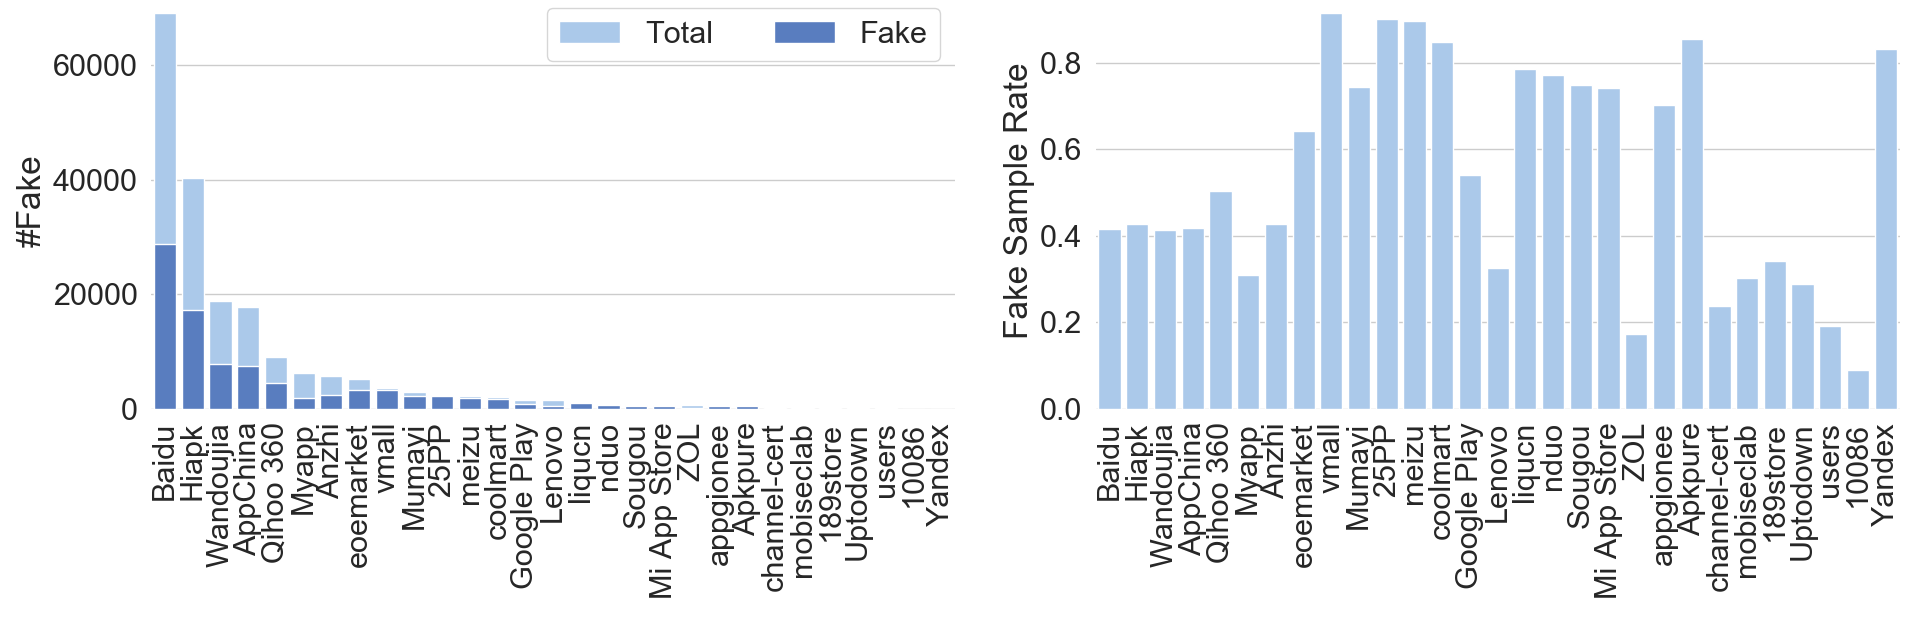
\includegraphics[width=\textwidth]{./Figures/edwin-Number_of_samples_collected_markets_3.png}
    \caption{从不同应用市场中收集到的应用数量以及各市场仿冒率}
    \label{fig:Sample_source}
\end{figure*}

左图显示,在本研究收集数据的所有29个应用来源中,从样本总数与仿冒样本数两个角度看,\texttt{百度手机助手}均提供了最多样本。
可将各渠道提供的样本量与市场规模相联系。
各个应用市场的仿冒率在右图呈现。


\texttt{百度手机助手}~\cite{Baiduappstore}和\texttt{安卓市场}~\cite{Hiapk}的仿冒率均约为40\%,在所有的29个渠道中处于中等水平,但由于源于该两个渠道样本基数最大,两者也提供了最多仿冒样本数。
由图中数据可得,应用市场的样本数量与仿冒率不直接相关。
然而,应用和市场的关系有可能对应用仿冒率产生影响:
本研究的50款目标应用中,有12款由腾讯公司开发,针对该12款应用进行仿冒率计算,可得结果如下:

\begin{table}[htbp]
    \renewcommand{\arraystretch}{1}
    \footnotesize
    \centering
    \caption{腾讯旗下12款应用于各大市场的仿冒率}
    \vspace{1mm}
    \begin{tabular}{l c c c c c c c c c}
        \toprule
        {\bf 应用市场}   & {\bf 百度} & {\bf 安卓市场} & {\bf 豌豆荚} & {\bf 应用汇} & {\bf 360} & {\bf 应用宝} & {\bf 安智} & {\bf 优亿} & {\bf 华为} \\
        \midrule
        {\bf 仿冒率(\%)} & 60.92      & 60.17          & 63.92        & 57.48        & 63.24     & 33.04        & 52.45      & 78.86      & 96.91      \\
        \bottomrule
    \end{tabular}
    \label{table:tencent_apps}
\end{table}

12款应用分别为QQ,微信,腾讯视频,腾讯手机管家,QQ音乐,开心消消乐,王者荣耀,QQ邮箱,QQ浏览器,腾讯新闻,应用宝和全民K歌。
应用宝为腾讯旗下应用市场,~\autoref{table:tencent_apps}中结果表明,应用宝中腾讯应用仿冒率明显比其他市场低。
有理由相信,应用宝对该12款应用相关的应用有较为严格的审核流程,有效遏制了该市场中与上述12款应用相关的仿冒应用。

结果表明,应用市场的规模与仿冒率无明显关联,但应用本身与市场的关系对仿冒率有影响。

\noindent{\bf RQ 2.2}:某应用的热度/更新频率/所在类别是否影响其对应仿冒率?

\subsection{其他因素对仿冒样本数量的影响}
% Accordingly, we hypothesize the following factors may influence the number of fake samples of an app:
除了市场本身之外,本节还假设以下这些因素可能会影响某款App对应的仿冒样本数量:

% \noindent{\bf Hypo 2.2:} The number of fake apps are closely related to how popular an app is.
{\bf 假设 2.2}:仿冒应用的数量与其对应的正版App的受欢迎程度有密切联系。

% \noindent{\bf Hypo 2.3:} Update frequency effects the number of fake samples.
{\bf 假设 2.3}:应用的更新频率影响着其对应仿冒应用的数量。

% \noindent{\bf Hypo 2.4:} Category is a factor influencing the fake sample number.
{\bf 假设 2.4}:App类别是影响仿冒应用数量的因素之一。

与三个假设对应的是三个研究问题:

% \noindent{\bf RQ 2.2}: Does the popularity of an app affect the number of its fake samples?
{\bf RQ 2.2}:一个App受欢迎的程度会影响对其仿冒的应用数量吗?

% \noindent{\bf RQ 2.3}: Does an app's update frequency influence its fake sample's number?
{\bf RQ 2.3}:一个App的更新频率会影响对其仿冒的应用数量吗?

% \noindent{\bf RQ 2.4}: Is the number of fake samples related to the app's category?
{\bf RQ 2.4}:一个App所在类别会影响对其仿冒的应用数量吗?

对于这三个研究问题,本节使用了皮尔逊积矩相关系数(Pearson product-moment correlation coefficient,简称PPMCC)来衡量应用数量和问题对应的几个维度的关联性。

% \noindent{\bf Answer to RQ 2.2.}
{\bf RQ 2.2. 结果}
% Intuitively, the more popular an app is, the more possible it would get shammed, for fake developers would mislead users to download their apps to gain profits.
从直觉上看,某款App越受欢迎,仿冒应用开发者就越有动机对其仿冒,然后诱导用户下载仿冒版本以获取利润。

% Note that each app has different amount of samples (including official samples and fake samples), processing our measurement directly based on the number of fake samples is incorrect.
要注意的是,每款目标App都有不同的样本数(无论是官方的或是仿冒的),所以在这里不能拿仿冒样本的数量直接作比较。
% To counteract this bias, each fake count should be regularize into a \textit{fake sample rate}, the rate of fake samples in all collected samples of an app.
为了消除偏差,本文将样本数量归一化,使用\autoref{equ:fake_rate_app}定义的仿冒率对每个目标App进行比较。
% Next, we employ a metric called \textit{Pearson product-moment correlation coefficient (PPMCC)} to reveal relativeness between an app's fake sample number and its popularity, which uses the regularized fake sample rates and monthly activeness indicators (MAI) obtained from Analysys~\cite{yiguanqianfan}.
接下来,本文使用了皮尔逊积矩相关系数来计算一款App被仿冒的严重程度与其热度是否具有相关性。
相关计算会使用上述的仿冒率和从易观千帆~\cite{yiguanqianfan}获取的App月度热度指数计算。

\begin{Def}
    皮尔逊积矩相关系数

    两个变量之间的皮尔逊相关系数定义为两个变量之间的协方差和标准差的商(\autoref{equ:PPMCC})。
\end{Def}
\begin{equation}
    p_x,_y = corr(X,Y)=\frac{cov(X,Y)}{\sigma_x\sigma_y}=\frac{E[(X-u_x)(Y-u_y)]}{\sigma_x\sigma_y}
    \label{equ:PPMCC}
\end{equation}
\vspace{0.5mm}

% This value ranges from -1 to 1, the closer the PPMCC value is to 0, the weaker correlation between the two factors is indicated.
\autoref{equ:PPMCC}的值域为$[-1, 1]$,该值越接近0,表示两个变量之间的相关关系越弱。
% Surprisingly, according to our data, the value of PPMCC between this two factors is 0.246, revealing that the fake sample number and an app's popularity only hold their relativeness on a weak level, which does not match our expectation.
出人意料的是,数据显示,两个因子之间的相关系数只有0.246。
这表明仿冒应用的数量和App的热度在相关性上只处于较弱水平,和本研究的预期并不符合。

% \noindent{\bf Answer to RQ 2.3.}
{\bf RQ 2.3. 结果}
% We assume the update frequency is related to the number of fake samples of an app, for updates can usually help keep a software from being attack.
本研究猜想更新频率有可能会与App被仿冒的次数相关联,因为升级通常会有漏洞修复等举措,可以帮助App免受攻击。
% The higher the update frequency is, the safer an app is supposed to be.
所以一款App的更新频率越高,其安全性能应该就会越好。

% To estimate the average update frequency of our target apps, the time when an app's official sample was crawled and when its latest official samples were crawled is marked.
为了评估一款目标App的平均更新频率,本研究标记了每个官方应用样本被发行时的时间,精确到日。
% The difference between them is then divided by the number of that app's existing version to obtain an update frequency, with unit day/version.
然后,再找到最新发布的那个样本和最早发布的那个样本,求出他们发行时间的差值的绝对值与版本数的商,即为平均更新频率(单位:天/版本)

% The result PPMCC value of 0.084 shows that the connection between an app's update frequency and its fake sample rate barely exists.
相关系数的计算结果表示,更新频率和仿冒数量之间的关联度只有0.084,意味着两者之间几乎没有关联。
% We attribute this result to two reasons:
本研究认为这个结果由两个原因导致:

% (1) The high update frequency (10 days/version on average for apps in our dataset) indicates app developers may not fix security issues in per update, weakening the function of update frequency as a security indicator.
1)在本研究的数据集中,每款App的平均更新间隔为10天/版本。
这个较高的更新频率表面开发者可能不会每次都在更新中修正安全性问题,从而削弱了更新频率作为安全性指标的功能。

% (2) A large portion of fake samples in our dataset are not derived from repackaging. To this end, fake developers can produce fakes regardless of how well the official apps are protected.
2)结合前文的结果,数据集中的大部分仿冒样本都不是重打包应用,而是仿冒应用开发者自行开发的。
因此,无论官方版本受到的保护程度如何,仿冒应用开发者都可以制造出对应的仿冒应用。

% \noindent{\bf Answer to RQ 2.4.}
{\bf RQ 2.4. 结果}
% Some categories are potentially more profitable than others.
某些App类别比其他类别更有可能带来收益。
% A report from the app marketing company LIFTOFF~\cite{LIFTOFF_report} forecasts gaming to be the next most billable area.
根据一份来自App营销机构LIFTOFF~\cite{LIFTOFF_report}的报告预测,在未来,\texttt{游戏}类有望成为带来最高收入的应用分类。

\begin{ThreePartTable}
    \centering
    \renewcommand{\arraystretch}{1.05}
    \footnotesize
    \setlength{\belowcaptionskip}{-5pt}
    \vspace{1mm}
    % \rowcolors{2}{gray!15}{white}
    \begin{longtable}{l l c c c c c c}
        \caption{目标App与其相关统计}\label{table:data-statistics}                                                                                                                                                        \\
        \toprule
        {\bf 应用名}                                 & {\bf 类别}     & \begin{tabular}[c]{@{}c@{}}{\bf 月度热} \\ {\bf 度指数} \end{tabular} & \begin{tabular}[c]{@{}c@{}}{\bf 更新频率} \\ {\bf (天/版本)} \end{tabular} & {\bf 样本总数} & \begin{tabular}[c]{@{}c@{}}{\bf 仿冒} \\ {\bf 样本数} \end{tabular} & {\bf 仿冒率} & \begin{tabular}[c]{@{}c@{}}{\bf 平均仿} \\ {\bf 冒延迟} \end{tabular} \\
        \midrule
        {\bf 微信}\tnote{*}                          & {\bf 社交网络} & {\bf 91.2K}                & {\bf 6.4}                  & {\bf 9248}     & {\bf 6447}                 & {\bf 69.7\%} & {\bf 12.1}                 \\
        \rowcolor{gray!15} {\bf QQ}\tnote{*}         & {\bf 社交网络} & {\bf 54.6K}                & {\bf 10.7}                 & {\bf 11167}    & {\bf 3780}                 & {\bf 33.8\%} & {\bf 9.2}                  \\
        爱奇艺                                       & 视频           & 53.5K                      & 6.4                        & 7586           & 3481                       & 45.9\%       & 9.3                        \\
        \rowcolor{gray!15} 支付宝                    & 生活           & 48.1K                      & 10.2                       & 983            & 231                        & 23.5\%       & 10.1                       \\
        {\bf 淘宝}\tnote{*}                          & {\bf 移动购物} & {\bf 47.5K}                & {\bf 7.0}                  & {\bf 6003}     & {\bf 3010}                 & {\bf 50.1\%} & {\bf 8.1}                  \\
        \rowcolor{gray!15} 腾讯视频                  & 视频           & 47.3K                      & 6.3                        & 1429           & 68                         & 4.8\%        & 10.7                       \\
        优酷                                         & 视频           & 40.9K                      & 7.3                        & 2058           & 262                        & 12.7\%       & 6.7                        \\
        {\bf 新浪微博}\tnote{*}                      & {\bf 社交网络} & {\bf 39.2K}                & {\bf 5.3}                  & {\bf 5947}     & {\bf 2715}                 & {\bf 45.7\%} & {\bf 5.7}                  \\
        \rowcolor{gray!15} WiFi万能钥匙              & 系统工具       & 36.4K                      & 3.1                        & 4808           & 2999                       & 62.4\%       & 3.0                        \\
        搜狗输入法                                   & 系统工具       & 33.3K                      & 11.0                       & 898            & 40                         & 4.5\%        & 21.8                       \\
        \rowcolor{gray!15} 百度                      & 资讯           & 32.4K                      & 11.1                       & 15651          & 3514                       & 22.5\%       & 12.8                       \\
        腾讯新闻                                     & 资讯           & 28.7K                      & 8.5                        & 1051           & 11                         & 1.0\%        & 8.9                        \\
        \rowcolor{gray!15} QQ浏览器                  & 资讯           & 27.8K                      & 5.6                        & 1369           & 43                         & 3.1\%        & 11.6                       \\
        今日头条                                     & 资讯           & 27.4K                      & 4.4                        & 3538           & 179                        & 5.1\%        & 5.6                        \\
        \rowcolor{gray!15} 应用宝                    & 应用市场       & 27K                        & 11.4                       & 2419           & 266                        & 11.0\%       & 11.6                       \\
        快手                                         & 视频           & 24.4K                      & 3.2                        & 8273           & 4270                       & 51.6\%       & 3.5                        \\
        \rowcolor{gray!15} 腾讯手机管家              & 系统工具       & 24.2K                      & 8.7                        & 2463           & 1340                       & 54.4\%       & 8.7                        \\
        高德地图                                     & 生活           & 24K                        & 6.5                        & 1225           & 51                         & 4.2\%        & 13.1                       \\
        \rowcolor{gray!15} 酷狗音乐                  & 音乐           & 23K                        & 8.6                        & 1313           & 122                        & 9.3\%        & 12.2                       \\
        QQ音乐                                       & 音乐           & 21.7K                      & 9.4                        & 1132           & 65                         & 5.7\%        & 14.6                       \\
        \rowcolor{gray!15} 百度地图                  & 生活           & 21.3K                      & 8.8                        & 2609           & 1438                       & 55.1\%       & 15.3                       \\
        抖音                                         & 视频           & 19.4K                      & 11.1                       & 317            & 12                         & 3.8\%        & 8.3                        \\
        \rowcolor{gray!15} {\bf 京东}\tnote{*}       & {\bf 移动购物} & {\bf 18.5K}                & {\bf 10.9}                 & {\bf 5000}     & {\bf 2377}                 & {\bf 47.5\%} & {\bf 12.3}                 \\
        UC浏览器                                     & 资讯           & 16.7K                      & 7.4                        & 4232           & 1624                       & 38.4\%       & 7.0                        \\
        \rowcolor{gray!15} 360手机卫士               & 系统工具       & 15.4K                      & 12.4                       & 3670           & 1423                       & 38.8\%       & 19.1                       \\
        全民K歌                                      & 音乐           & 14.7K                      & 21.1                       & 618            & 215                        & 34.8\%       & 17.3                       \\
        \rowcolor{gray!15} 美团                      & 生活           & 13K                        & 8.0                        & 4752           & 1415                       & 29.8\%       & 6.9                        \\
        {\bf 拼多多}\tnote{*}                        & {\bf 移动购物} & {\bf 12.9K}                & {\bf 6.6}                  & {\bf 2327}     & {\bf 551}                  & {\bf 23.7\%} & {\bf 7.8}                  \\
        \rowcolor{gray!15} {\bf 王者荣耀}\tnote{*}   & {\bf 游戏}     & {\bf 12.5K}                & {\bf 15.5}                 & {\bf 2350}     & {\bf 1319}                 & {\bf 56.1\%} & {\bf 12.3}                 \\
        美图秀秀                                     & 摄影录像       & 12.4K                      & 5.4                        & 1705           & 784                        & 46.0\%       & 5.8                        \\
        \rowcolor{gray!15} 火山小视频                & 视频           & 12.2K                      & 11.9                       & 410            & 16                         & 3.9\%        & 9.6                        \\
        墨迹天气                                     & 生活           & 12K                        & 4.2                        & 10081          & 7093                       & 70.4\%       & 4.7                        \\
        \rowcolor{gray!15} 滴滴出行                  & 生活           & 11.8K                      & 8.6                        & 943            & 117                        & 12.4\%       & 7.0                        \\
        华为应用市场                                 & 应用市场       & 11.8K                      & N/A                        & 0              & 0                          & 0.0\%        & N/A                        \\
        \rowcolor{gray!15} {\bf 开心消消乐}\tnote{*} & {\bf 游戏}     & {\bf 11.2K}                & {\bf 19.7}                 & {\bf 2406}     & {\bf 1738}                 & {\bf 72.2\%} & {\bf 20.6}                 \\
        酷我音乐盒                                   & 音乐           & 11K                        & 2.9                        & 3778           & 69                         & 1.8\%        & 4.2                        \\
        \rowcolor{gray!15} 西瓜视频                  & 视频           & 11K                        & 11.5                       & 866            & 100                        & 11.5\%       & 8.8                        \\
        OPPO应用商店                                 & 应用市场       & 10.8K                      & N/A                        & 0              & 0                          & 0.0\%        & N/A                        \\
        \rowcolor{gray!15} 猎豹清理大师              & 系统工具       & 9.9K                       & 10.3                       & 1803           & 388                        & 21.5\%       & 13.5                       \\
        360清理大师                                  & 系统工具       & 9.6K                       & 17.3                       & 327            & 8                          & 2.4\%        & 8.5                        \\
        \rowcolor{gray!15} 360手机助手               & 应用市场       & 9.2K                       & 7.6                        & 1616           & 137                        & 8.5\%        & 8.4                        \\
        WiFi管家                                     & 系统工具       & 8.8K                       & 19.5                       & 1636           & 658                        & 40.2\%       & 15.7                       \\
        \rowcolor{gray!15} 讯飞输入法                & 系统工具       & 8.6K                       & 6.0                        & 1451           & 8                          & 0.6\%        & 10.1                       \\
        百度手机助手                                 & 应用市场       & 8.2K                       & 11.4                       & 3849           & 437                        & 11.4\%       & 14.5                       \\
        \rowcolor{gray!15} 小米应用市场              & 应用市场       & 7.8K                       & N/A                        & 0              & 0                          & 0.0\%        & N/A                        \\
        {\bf WPS Office}\tnote{*}                    & {\bf 商务办公} & {\bf 7.4K}                 & {\bf 6.0}                  & {\bf 1152}     & {\bf 69}                   & {\bf 6.0\%}  & {\bf 7.8}                  \\
        \rowcolor{gray!15} 美颜相机                  & 摄影录像       & 7.1K                       & 5.3                        & 1600           & 691                        & 43.2\%       & 6.3                        \\
        网易云音乐                                   & 音乐           & 7K                         & 10.5                       & 616            & 6                          & 1.0\%        & 12.2                       \\
        \rowcolor{gray!15} 网易新闻                  & 资讯           & 6.7K                       & 7.0                        & 1441           & 93                         & 6.5\%        & 5.0                        \\
        {\bf QQ邮箱}\tnote{*}                        & {\bf 商务办公} & {\bf 6.6K}                 & {\bf 16.4}                 & {\bf 520}      & {\bf 11}                   & {\bf 2.1\%}  & {\bf 10.4}                 \\
        \bottomrule
    \end{longtable}
    \vspace{-4mm}
    \begin{tablenotes}
        % \item[*] Detailed descriptions are given in {\bf Answer to RQ 2.4}
        \item[*] 详情会在{\bf RQ 2.4. 结果}中给出
    \end{tablenotes}
\end{ThreePartTable}

% Our 50 target apps are divided into 11 categories according to their functionalities, Table~\autoref{table:data-statistics} shows these categories and their corresponding fake sample rate.
根据应用功能划分,本研究的50款目标App可以被分为11个类别。
\autoref{table:data-statistics}按每款App的热度排序,展示了每款App的类别和他们的仿冒率,同时还有他们的更新频率、关联样本总数等数据。
% In the same category, the difference between apps on fake rate lies in an acceptable range.
在相同的类别下,多数应用之间的仿冒率差值都位置在一个合适的水平。
% Without doubt, entertainment related categories like \texttt{游戏} and \texttt{Social Network} attract more fake samples.
毫无疑问地,娱乐方向的类别(比如\texttt{游戏}和\texttt{社交网络})吸引了更多仿冒应用开发者对其仿冒。
% Another field, \texttt{Online shopping}, has also gained special love from fake developers because online shopping is rapidly developing in China.
而另一个类别\texttt{移动购物}也特别受到了仿冒应用开发者的``关照'',因为移动购物在中国也正在快速地发展。
% Relatively, \texttt{商务办公} is not that attractive to fake developers, the average fake sample rate of this filed is only 4.05\%.
相对来说,商务方向的\texttt{商务办公}分类的应用就不是那么地吸引仿冒应用开发者了,这个领域下的App平均仿冒率只有4.05\%。
% Apps in these four categories are marked in bold in the table.
上述四个类别的应用都在表中被加粗标识,读者可以自行查阅。

% The result matches the observation in our daily life, people always tend to use mobile devices for entertainment instead of business purpose.
这个结果与日常生活中可观察到的结果相符,比起商务类用途,普罗大众更倾向于使用移动设备用作娱乐用途,消遣时间。
% It's pretty interesting to discover that the number of fake samples in a way reflects how people use their phone in their daily lives.
仿冒应用的数量从某种角度上反映了人们在日常生活中如何使用移动设备,这是个十分有趣的发现。

% \noindent{\bf Case study 2.} \emph{Fake samples in different gaming apps}
\subsection{案例 2. 游戏类别下的仿冒应用}

% Gaming apps in our target app list (i.e. \texttt{\small ArenaofValor} and \texttt{\small HappyElements}) attract a number of fake samples.
正如\autoref{table:data-statistics}中数据所示,\texttt{游戏}类应用(\texttt{王者荣耀}和\texttt{开心消消乐})吸引了大批的仿冒应用样本。
% To figure out what do these samples look like, we randomly downloaded some of the fake samples of the 2 gaming apps (7 samples for each) and installed them on our testing device.
出于性能考虑,此处的数据中只提取了APK包的基本信息,并没有对收集到的每个APK文件进行详细的分析。
因此,为了弄清楚这些仿冒应用究竟是怎么样的,本研究随机从这两款游戏App的仿冒样本中选择了一些样本(每款应用选择7个仿冒样本),然后将这些样本安装到了实验设备上。

% Fig.~\ref{fig:screenshot_all} shows how these samples look like on a real Android phone, official apps are marked with green frames.
\autoref{fig:screenshot_all}展示了这些样本在真实的Android设备上安装之后的实际外观。
官方渠道下载的正版App在图片中由绿色边框标记出。
% Apparently, fake samples have either a similar name or a similar icon to official ones.
明显地,与官方应用相比,仿冒应用或者有一个和官方应用名十分相似的应用名,或者在图标上和官方相近甚至相同。

\begin{figure}[htbp]
    \centering
    \subfloat[两种游戏App与其仿冒\label{fig:screenshot_all}]{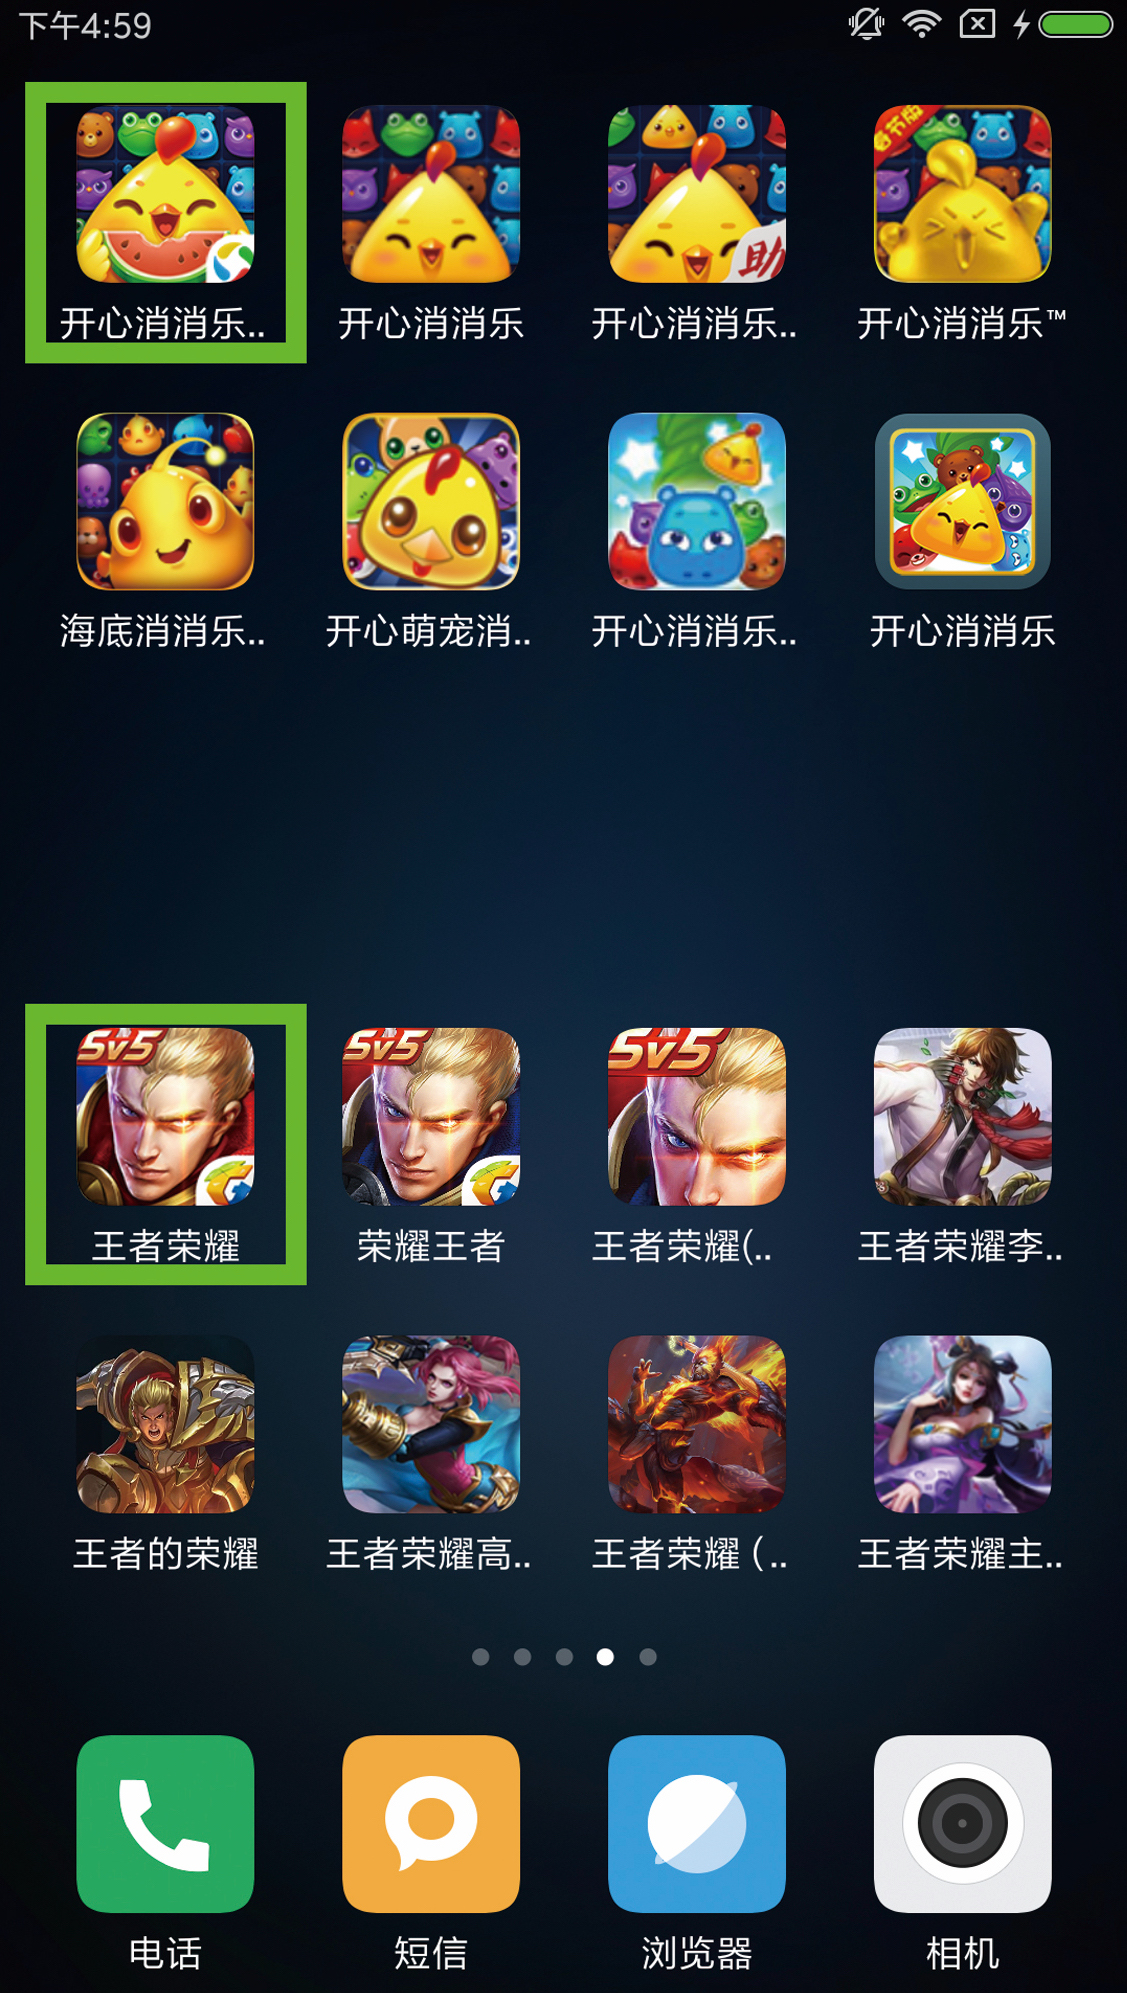
\includegraphics[width=0.3\textwidth]{./Figures/edwin-screenshot1.jpg}}\hfill
    \subfloat[正版\textit{\small 开心消消乐}\label{fig:screenshot_official}]{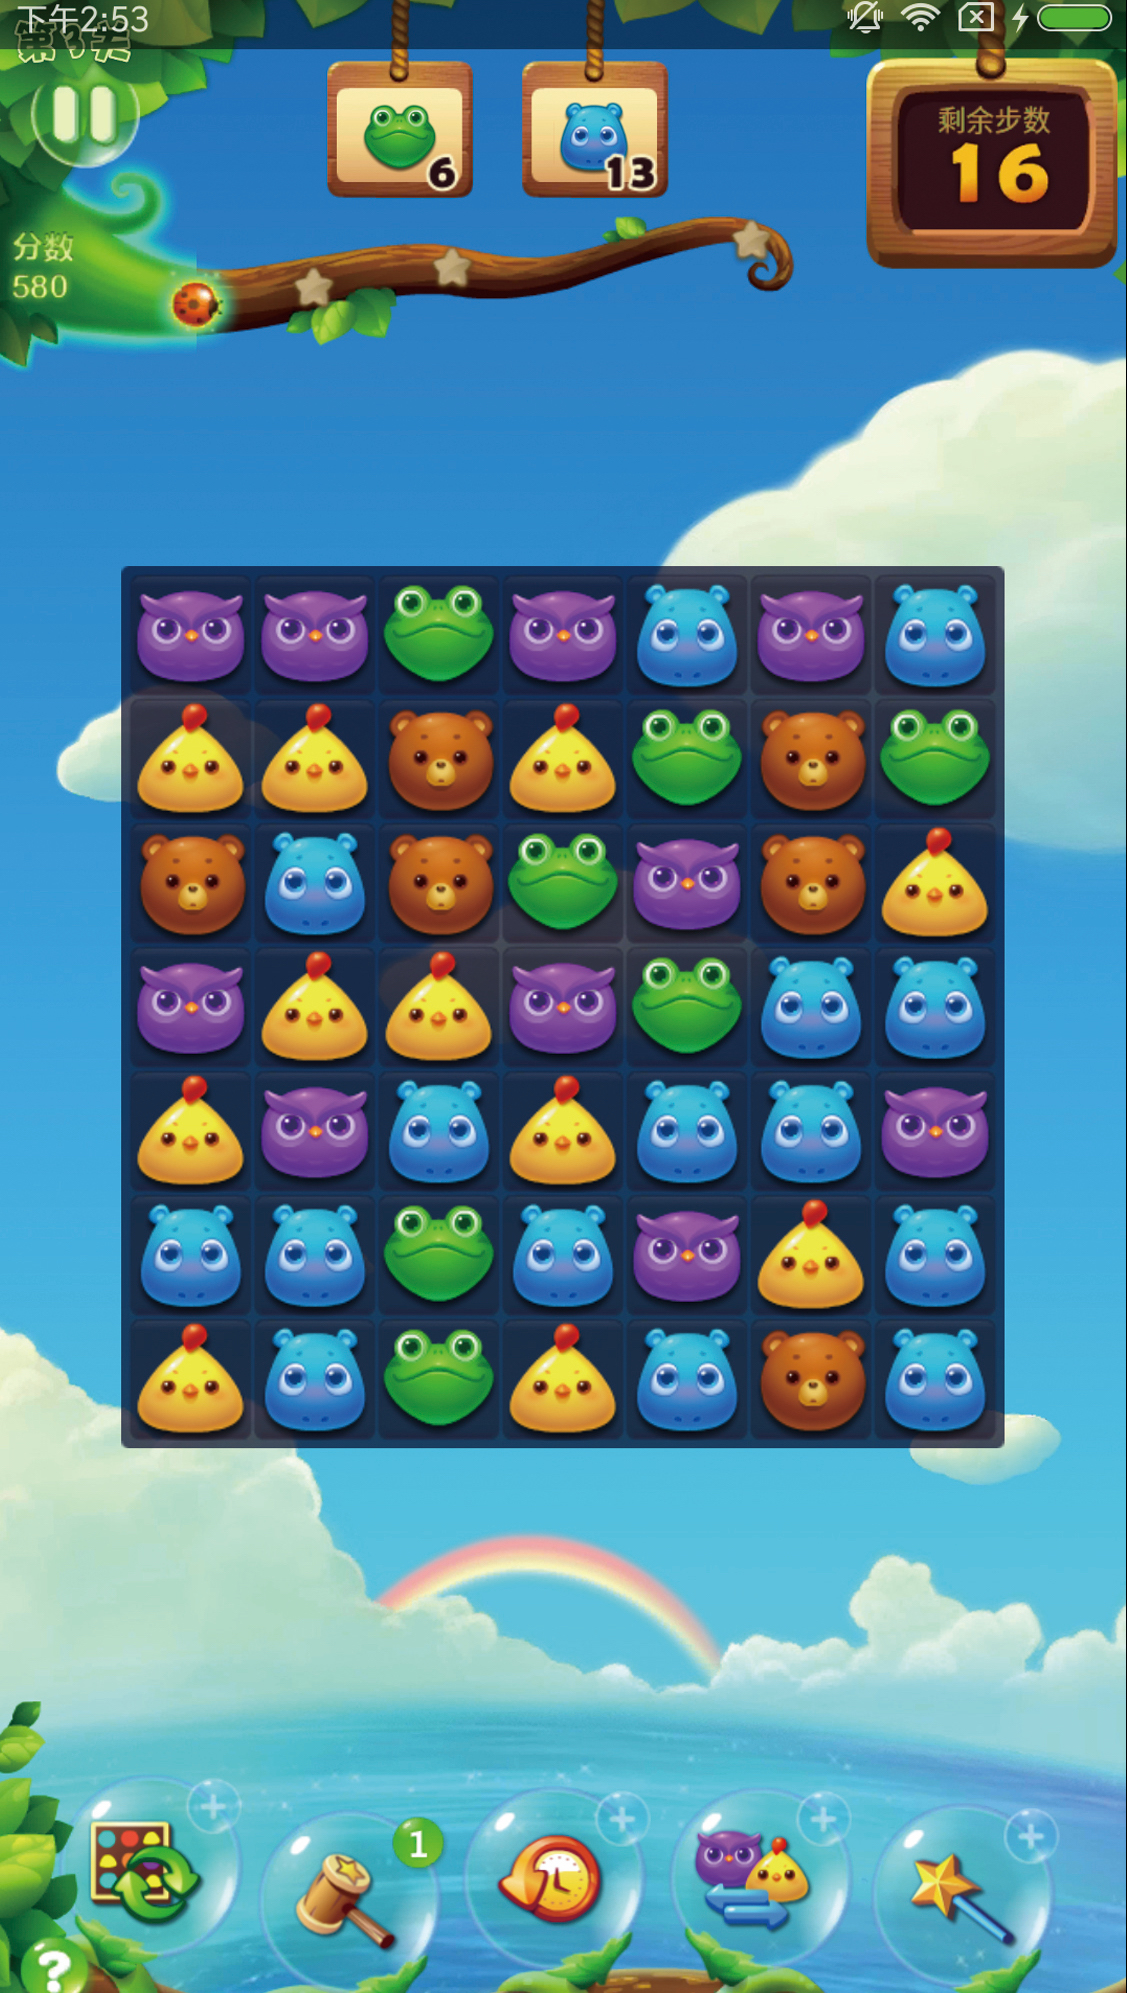
\includegraphics[width=0.3\textwidth]{./Figures/edwin-screenshot2.jpg}}\hfill
    \subfloat[仿冒版\textit{\small 开心消消乐}\label{fig:screenshot_fake}]{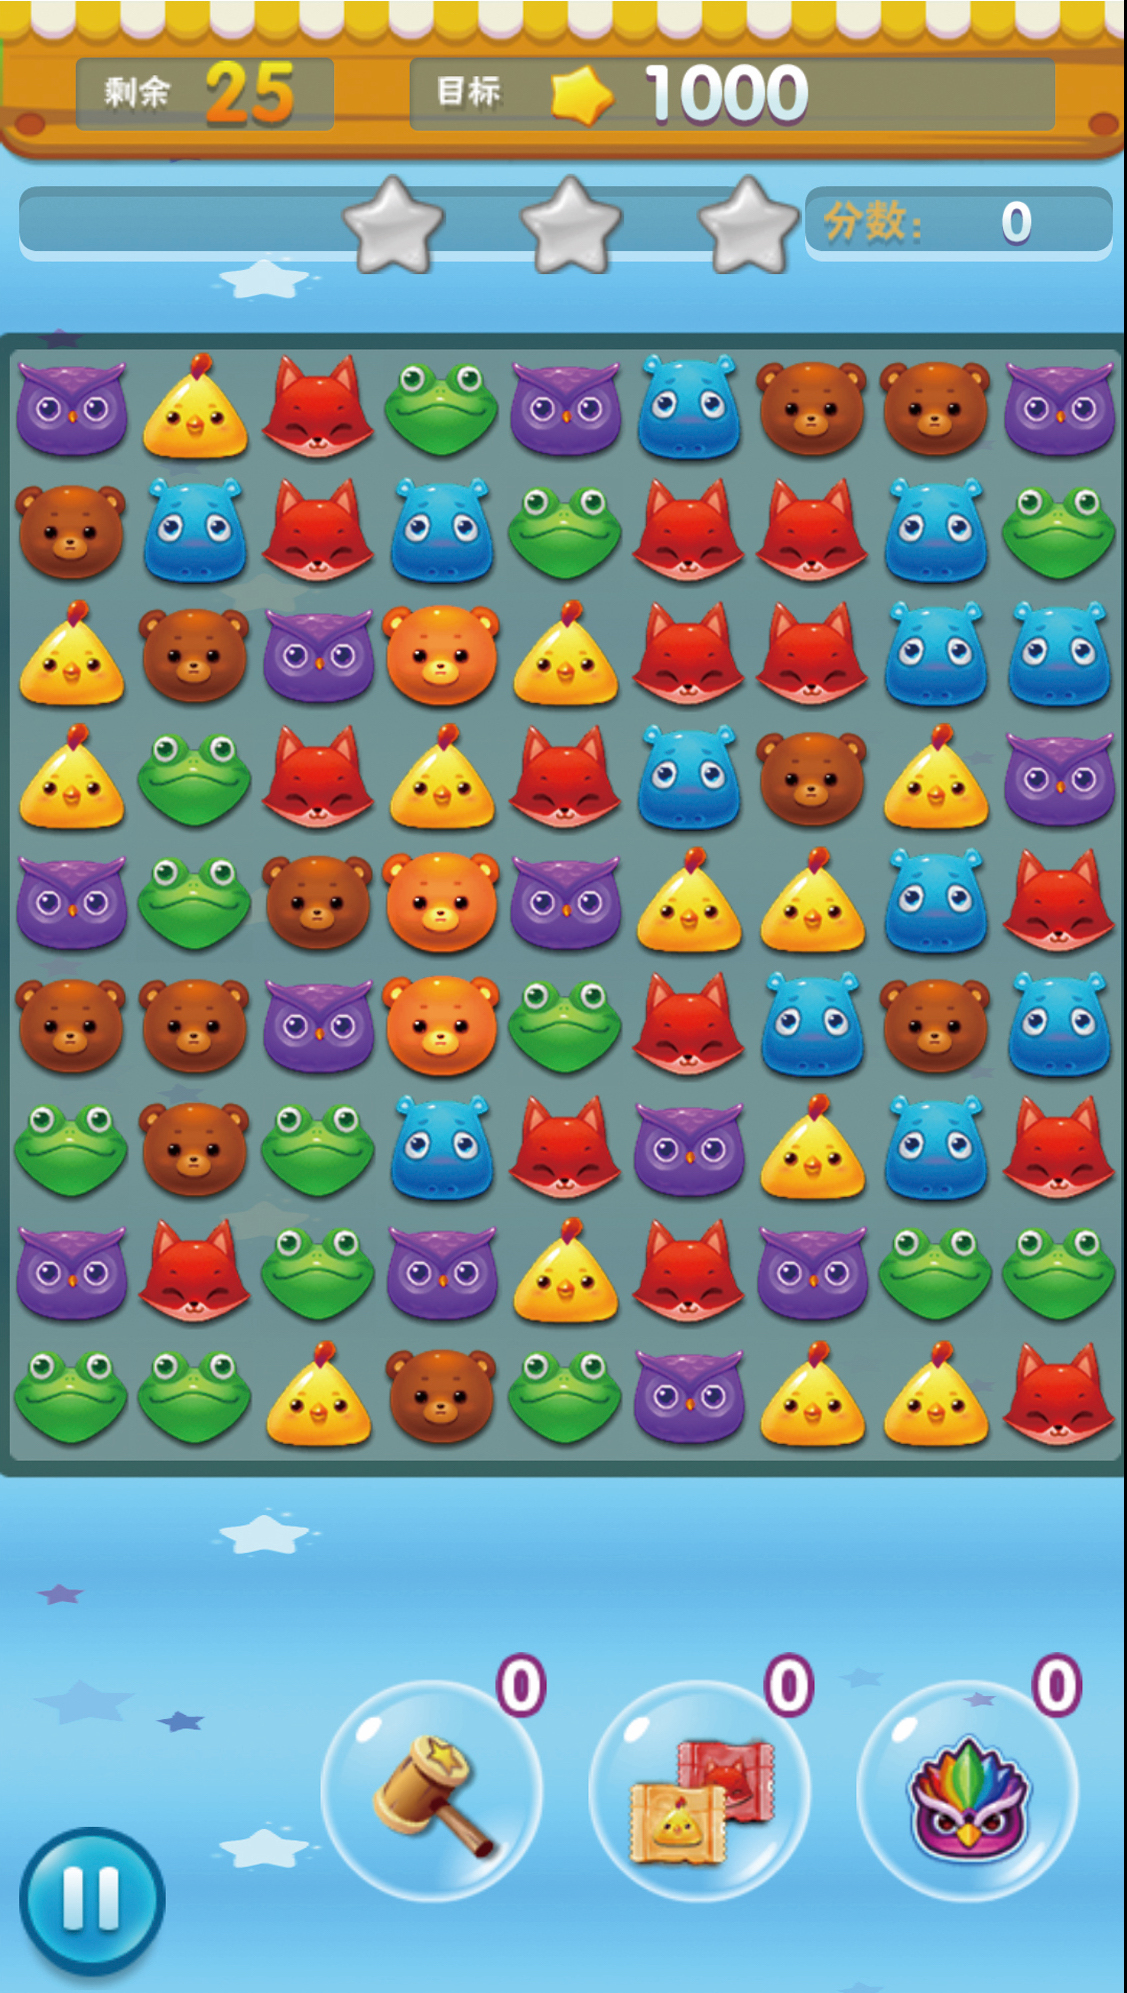
\includegraphics[width=0.3\textwidth]{./Figures/edwin-screenshot3.jpg}}\hfill
    \caption{游戏类App及其仿冒样本}
\end{figure}

% We even ran these apps on our device.
本研究在测试设备上实际运行了上述安装的14个仿冒样本,然后拿它们和原版的应用对比。
测试使用的设备为高配版小米5手机,搭载的CPU为最高主频2.15GHz的骁龙820处理器,3GB内存,64GB机身存储,安装的Android系统版本为Android 6.0(Android Marshmallow,API 23)。

% Screenshots were captured when we ran one of the fake samples (see Fig.~\ref{fig:screenshot_fake}) and the official sample (Fig.~\ref{fig:screenshot_official}).
\autoref{fig:screenshot_official}和\autoref{fig:screenshot_fake}分别是在测试设备上运行官方版本的\texttt{开心消消乐}和其中一个仿冒版的\texttt{开心消消乐}时的系统截屏。
不难看出,两款应用的外观是十分相像的。
本研究在测试时发现,两款游戏内部的玩法、实际操作逻辑也一模一样。
如果不是事先知道了哪一款应用是来自官方渠道下载的正版,一般的应用开发者也未必可判别两个应用的真伪,更不必说是从应用市场搜索结果中找到这些结果的普通用户了。

% As a result, we found that 4 fake samples of \texttt{\small HappyElements} are actually games that are similar to the official one (one is a repackaged app with high confidence), 2 are raiders on the game and the last one crashed when it was launched.
而这并不是唯一的案例。作为结果,本研究发现7款\texttt{开心消消乐}的仿冒样本中,有4款是与官方样本十分相似的游戏(其中一个十分可能是经过重打包技术处理的应用),2款声称自己是``系统攻略'',还有1款在运行时闪退,无法在测试设备上实际运行。
% 3 out of the 4 fake games pop up alert windows in the game to require users for In-App purchase, which is very possible to cause unwilling cost.
在4款仿冒游戏中,3款都在游戏中不时自动弹出游戏内购窗口,要求玩家购买道具,十分可能导致玩家不想要的花费。
% All 7 samples are reported to be malicious on \textsc{Virustotal}~\cite{virustotal}.
而所有7个仿冒样本都在\textsc{Virustotal}~\cite{virustotal}中被报告为恶意应用。

% Fake samples on \texttt{\small ArenaofValor}, in contrast, barely have functionalities like the official one.
相比之下,\texttt{王者荣耀}的仿冒样本内容就与官方应用大相径庭了。
% 3 of those samples are wallpaper setters and the rest 4 are simply puzzle games.
在7款被安装到测试设备的仿冒样本中,有3款是壁纸浏览器,里面包含了几张游戏内人物的插画,可以在应用内将这些插画设置成系统的桌面壁纸;
而余下四个是简单的拼图游戏,里面同样包含了王者荣耀游戏人物的插画,应用内容就是简单地把被打乱的插画拼图恢复原状。
% Virustotal reports 6 out of the 7 samples as malware, the last one is claimed as potentially unwanted program (PUP).
Virustotal的结果显示,7款仿冒样本中,有6款是恶意软件,涵盖了木马病毒、广告软件等类型,而余下的一款则被报告为潜在有害程序(Potentially Unwanted Program,简称PUP)。
PUP通常在用户不知情或者不愿意的情况下,通过静默安装或者捆绑安装的形式被安装在系统中。
尽管这种软件不一定包含恶意代码,但其动机十分可疑。

% We determine it is the difficulty to imitate the official app's functionality that brings about this phenomenon.
本研究认为,这种现象是由模仿正版应用功能的难易程度带来的。
% The core implementation of multiplayer online battle arena (MOBA) games like \texttt{\small ArenaofValor} is much more complicated than that in \texttt{\small HappyElements}.
只从技术角度看,像\texttt{王者荣耀}这样的多人在线战斗竞技场(Multiplayer Online Battle Arena,简称MOBA)游戏核心难度明显要比\texttt{开心消消乐}这样的益智类游戏要高得多。
一款MOBA游戏除了要解决支持运行运行的物理引擎之外,还要实现聊天系统、在线匹配、负载均衡等业务,更加不必说背后的人物设计技能平衡等更深入的话题了;而一款益智类三三消游戏的核心逻辑就只在于元素三连的判定和随机新出现的元素,再加上道具系统就差不多可以包装成一个完整的游戏推出。

% What it costs to develop a complex game like \texttt{\small ArenaofValor} is exorbitant for a fake developer.
因此,就算不考虑后续的维护问题,要开发一款像\texttt{王者荣耀}这样的复杂游戏,对仿冒应用开发者来说明显是成本过高的。
但由于这款游戏本身具有超高的热度,可能带来巨大的收益,所以仿冒应用开发者会为了蹭上热度而开发外观相似、内容完全不符的仿冒样本。
相比之下,\texttt{开心消消乐}由于开发难度相对较小,所以仿冒应用开发者会愿意开发一个内容相似的应用,再通过内购陷阱等手段收取效益。
这两款App透露出了仿冒应用开发者在仿冒方面两个截然不同的思路。

% Therefore, we can infer another reason why apps in \texttt{\small productivity} category gain a low fake sample rate:
本文在\secref{sec:quantitativeStudy}中观察到的\texttt{商务办公}类别有较低仿冒率也可能是类似原因导致的结果。
% Unlike games, on one hand, productivity tools are less likely to have peripheral products (like wallpaper setter mentioned above);
一方面,\texttt{商务办公}类的工具核心逻辑比较复杂,对仿冒开发者来说并不是一个有利可图的最佳选项;
% On the other hand, the inevitably laborious developing procedure also prevents the tools themselves from being shammed.
另外,这类应用也不像\texttt{游戏}一样会衍生出周边产品(比如\texttt{王者荣耀}的游戏人物就会有不少插画),仿冒应用开发者也没办法从这方面入手蹭热度。
结合两个原因,\texttt{商务办公}类的应用自然不会引起仿冒应用开发者的太多兴趣。

\vspace{5mm}
\noindent\fbox{
    \parbox{0.95\linewidth}{
        % \textbf{Remark 2}: As revealed by statistics, the number of samples returned from an app store does not imply a fake rate.
        \textbf{本节小结}: 正如由本文的统计和计算揭示的那样,从一个应用市场中能找到的应用样本数量并不能与应用商店的仿冒率相对应。
        % Additionally, the relationship between apps and market itself influences the number of fake samples from that market.
        此外,App本身与应用市场的关系也会影响到市场中对应App仿冒样本的数量。
        % To our surprise, an app's update frequency is not tightly correlated with its fake rate.
        出人意料的是,App的更新频率并没有与仿冒率相关联。
        % We owe this to the fact that apps are updated too frequently and that repackaged samples are of minority in our dataset.
        本研究认为这是由于应用更新频率太高、而且重打包应用在本研究的数据集中占少数而导致的结果。
        % We further observe that ``category'' as a factor has greater influence on the number of fake samples of an app than ``popularity'' and ``update frequency''.
        本文进一步观测到,与\texttt{更新频率}和\texttt{应用热度}相比,\texttt{应用分类}这一因素对App的仿冒率有更大的影响。
        案例分析从游戏类别的仿冒应用入手,说明了仿冒应用开发者对不同应用会采用不同仿冒策略。
    }
}

\section{相关工作}

\section{本章小结与实用建议}

